\documentclass{article}
\usepackage{a4}
\usepackage{url}
\usepackage{moreverb}
% graphicx package, useful for including eps and pdf graphics
% include graphics with the command \includegraphics
\usepackage{graphicx}
\usepackage{tabularx}
\begin{document}

\newcommand{\PALMA}{{\sl PALMA}}
\newcommand{\PALMapper}{{\sl PALMapper}}
\newcommand{\GM}{{\sl GenomeMapper}}
\newcommand{\Galaxy}{{\sl Galaxy}}
\newcommand{\mGene}{{\sl mGene}}
\newcommand{\ASP}{{\sl ASP}}
\newcommand{\evaluationToolbox}{{\sl evaluationToolbox}}
\newcommand{\QP}{{\sl QPALMA}}
\newcommand{\QPA}{{\sl QPALMA alignment algorithm }}
\newcommand{\QPH}{{\sl QPALMA approximation }}
\newcommand{\QPP}{{\sl QPALMA pipeline }}
\newcommand{\qparam}[1]{{\bf #1}}



\setlength{\parindent}{0cm}


\title{PALMapper Documentation}
\author{G\'eraldine Jean}
\date{December 2010}

\maketitle
%
%
%

\section{Overview}
\label{sec:overview}

\PALMapper{}~\cite{Palmapper} is the fusion of the short read mapper
\GM{}~\cite{GenomeMapper} and the short read aligner
\QP{}~\cite{DeBona08}. This is an easy-to-use and flexible tool 
to accurately and efficiently align both transcriptome reads (spliced 
and unspliced) from RNA-Seq experiments against a reference
genome. \PALMapper{} is able to take advantage of read-quality 
information by using the efficient training algorithm of \QP{}. It is
additionally able to benefit from computational splice-site
predictions which can be computed via
\mGene{}~\cite{Schweikertetal09,Schweikertetal09b} or
\ASP{}~\cite{Sonnenburgetal07} to improve the alignment accuracy.\\ 
This documentation describes how to install \PALMapper{} and how to
use it on the command-line based on (a) the reference genome, (b) a 
set of RNA-seq reads and (c) a \QP{} parameter file (obtained by
training \QP{}). \PALMapper{} can also be used through a Web service,
which is a customized version of the Galaxy
framework~\cite{Galaxy1,Galaxy2,Galaxy3}. For further detail, a
comprehensive tutorial~\cite{Palmapper} about 
training \QP{}, aligning with \PALMapper{}, evaluating and visualizing
the resulting alignments is available in Current Protocols in
Bioinformatics. 

For further information, you may contact:
\begin{center}
Gunnar R\"atsch (Gunnar.Raetsch@tuebingen.mpg.de)\\
G\'eraldine Jean (gjean@tuebingen.mpg.de)
\end{center}


\section{Installation}
\label{sec:installation}

\subsection{Dependencies}
\label{sec:dependencies}
\PALMapper{} is designed to run on \emph{Linux}/UNIX or \emph{Mac OS X} platforms and
can be downloaded at this address:\\
\url{http://ftp.tuebingen.mpg.de/pub/fml/raetsch-lab/software}.\\
This package is distributed under the GNU Public License (GPL). Read
the license before installation. The programs are distributed as C++
source. The memory requirement of \PALMapper{} depends on which kind of index is used:
\begin{itemize}
\item GenomeMapper index: it needs about seven times the genome size
  of main memory (four times for the index, about two times for
  splice-site predictions, and one time the genome size as working
  memory). In this case, \PALMapper{} requires about 21 GB of memory
  for the human genome. 
\item Burrows-Wheeler transform (bwt)-based index. %TODO
\end{itemize}
The machine’s architecture does not significantly influence the memory requirement for
these program.\\

The software package has the following dependencies on other packages:
\begin{itemize}
\item C++ compiler, for instance GNU C/C++ Compiler gcc/g++
(http://www.gnu.org). For other compilers, the compiler flags may need to be
adapted in the Makefile file.
\item Standard programs, such as \texttt{wget}, \texttt{make}, etc.
\item SAMtools for manipulating alignments in the SAM format
(http://samtools.sourceforge.net/).
\end{itemize}

\subsection{Step by step installation guide}
\label{sec:installguide}

\begin{enumerate}
\item Go to \url{http://ftp.tuebingen.mpg.de/pub/fml/raetsch-lab/software/}
    and download the package \texttt{palmapper/palmapper-0.4.tar.gz}
    to the home directory. 

\item Extract the tar-gzipped file in your home directory as follows:
\begin{verbatim}user:~$ cd
user:~$ tar zxvf palmapper-0.4.tar.gz\end{verbatim}
This command decompresses and unpacks the different files contained in
the archive to a directory named \texttt{palmapper-0.4}.

\item Compile \PALMapper{} by typing:
\begin{verbatim}user:~$ cd palmapper-0.4
user:~/palmapper-0.4$ make\end{verbatim}
Two binary files are created in the working directory: \texttt{palmapper} (the
mapping program) and \texttt{pmindex} (genome array-based index
builder). An other binary file named \texttt{bwa} is created under
\texttt{src/bwa/} and is used for building a genome bwt-based index.
\end{enumerate}

\section{Generating alignments with PALMapper}
\label{sec:aligning}

This section shows how to use \PALMapper{} for generating both unspliced
and spliced alignments for a set of RNA-Seq reads on the
command-line with the consideration that \QP{}~\cite{DeBona08} has
been already trained and optionally splice sites have been predicted
(see section~\ref{sec:inputfile} about input files) for the organism
of interest. Finally, this section describes a testcase suite included in
the package that checks whether \PALMapper{} gives the expected
results. The Galaxy version of \PALMapper{} is briefly described in
section~\ref{sec:aligninggal}. 

\subsection{Input files}
\label{sec:inputfile}
Aligning with \PALMapper{} needs the following files: 
\begin{itemize}
\item Genome sequence in FASTA format
\item Read data to align in Sanger FASTQ format (see section
  \ref{sec:readfile} for Sanger FASTQ format).
\item Genome annotation in GFF3 format (optional).
\item Donor and acceptor splice-site predictions in SPF format and
corresponding binary files (optional; see section
\ref{sec:splicescoresfile} for BSPF format). There are two ways for
obtaining these files: splice site predictions can be computed for a
given genome via an appropriate tool (see
\mGene{}~\cite{Schweikertetal09,Schweikertetal09b} or
\ASP{}~\cite{Sonnenburgetal07} for example). It can be done using the
Galaxy system (\url{http://galaxy.tuebingen.mpg.de/}) and then
downloaded for local use. Alternatively, the user can directly
download precomputed splice site predictions for a growing list of
organisms at
\url{http://ftp.tuebingen.mpg.de/pub/fml/raetsch-lab/predictions/splice}. In
this case, the splice site predictions have to be used together
with the corresponding version of genome sequence. Splice-site
predictions and the corresponding version of the genome can be easily
downloaded by running the command: 
\begin{verbatim}
user:~/palmapper-0.4/splice_predictions$ make <organism>
\end{verbatim}
where \texttt{<organism>} is the name of the organism of interest.\\
The user may also disable the use of splice site predictions by using
\texttt{-no-ss-pred} parameter in the way explained in step 2 below.
\item \QP{} parameter file (see
  Figure~\ref{fig:qp_parameter_file}). This file is obtained by
  training \QP{} (for more information, consult the comprehensive tutorial
  paper about \PALMapper{}~\cite{Palmapper}). Pretrained \QP{}
  parameter files for use with \PALMapper{} are located 
in: \texttt{~/palmapper-0.4/qpalma\_parameters}. Be sure to read the
README file in the same directory for more information.
\end{itemize}

\begin{figure}[h!]
\begin{center}
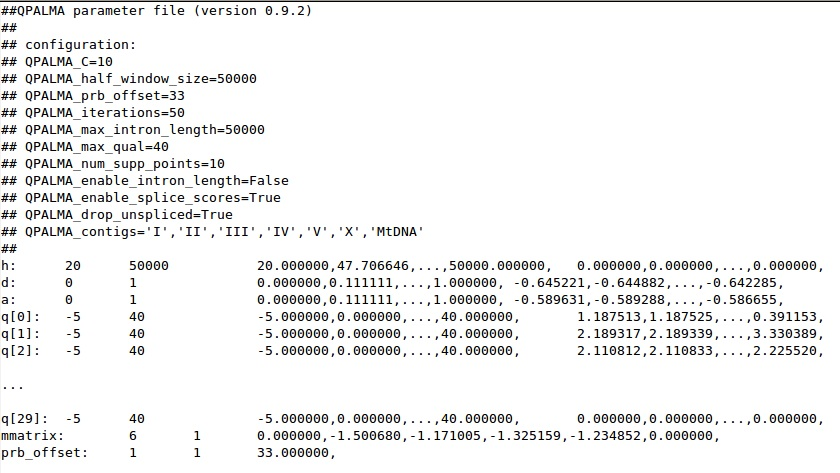
\includegraphics[width=\textwidth]{QPALMAFile.jpg}
\end{center}
\caption{Example of a \QP{} parameter file generated during the training
  phase of \QP{}. The first lines starting with $\#\#$ characters
  describe the parameters used for generating this file. The following
  lines represent the piece-wise linear functions for intron length (h),
  donor splice sites (d), acceptor splice sites (a) and edit operations
  for match/mismatch/gap on read (q). Each piece-wise linear function is
  defined by the range of possible x-values (length for h, splice site
  predictions for d and a, quality for q) which is followed by the
  values for all support points (first, x-values separated by commas
  then, after a space, y-values separated by commas
  too). \texttt{mmatrix} defines fixed scores for a gap on DNA according
  to possible aligned base in read. Finally, \texttt{prb\_offset} is the
  quality offset for determining the quality value from the ASCII
  quality character.}
\label{fig:qp_parameter_file}
\end{figure}

\subsection{Aligning with PALMapper on the command-line}
\label{sec:aligningcl}

\begin{enumerate}
\item Create an index of the reference genome:\\
\PALMapper{} offers the possibility to use two different kinds of
index for the reference genome: array-based and bwt-based indexes. The
first one uses more space but provides a better runtime especially for
small genomes. We advise the user to
use array-based index for genomes of small size (\emph{C. Elegans} for
instance) and the bwt-based index for large genomes as \emph{Human}.
\begin{itemize}
\item[a.] Create an array-based index:
\begin{verbatim}
user:~$ cd palmapper-0.4/
user:~/palmapper-0.4$ ./pmindex -i <genome_file> -s <index_size> -v
\end{verbatim}
where \texttt{<index\_size>} is the seed length used during indexing
(e.g., 13). This creates 4 files the prefix of which is
\texttt{<genome\_file>}:
\begin{itemize}
\item \texttt{<genome\_file>.cid}: chromosome index file
\item \texttt{<genome\_file>.mta}: meta index file
\item \texttt{<genome\_file>.mfd}: forward index file
\item \texttt{<genome\_file>.mrc}: reverse index file
\end{itemize}

\item [b.] Create a bwt-based index:
\begin{verbatim}
user:~$ cd palmapper-0.4/src/bwa
user:~/palmapper-0.4/src/bwa$ ./bwa index <genome_file>
\end{verbatim}
This creates 4 files the prefix of which is \texttt{<genome\_file>}:
\begin{itemize}
\item \texttt{<genome\_file>.bwt}: forward index file
\item \texttt{<genome\_file>.rbwt}: reverse index file
\item \texttt{<genome\_file>.sa}: suffix array for forward index
\item \texttt{<genome\_file>.rsa}: reversed suffix array for reverse
  index file
\end{itemize}
\end{itemize}

\item Use the command below to run \PALMapper{} within the working directory. The
command provided here is a generic one for computing both unspliced and spliced
alignments (spliced via \texttt{-S} option), and the user should
revise the options described in section~\ref{sec:settings} for best results.
\begin{verbatim}
user:~/palmapper-0.4$ ./palmapper -i <genome_file> -q <read_file> \
[OPTIONS_PALMAPPER] -S -qpalma <qpalma_param_file> \
-acc <acc_pred_file> -don <don_acc_file> -o <out_mapped_file> \
-u <out_unmapped_file> [OPTIONS_QPALMA]
\end{verbatim}

where:
\begin{itemize}
\item \texttt{<genome\_file>} is the path to the genome sequence file.
\item \texttt{<read\_file>} is the path to the genome read data file.
\item \texttt{<qpalma\_param\_file>} is the path to the \QP{} parameter file.
\item \texttt{<acc\_pred\_file>}, \texttt{<don\_pred\_file>} are the paths to acceptor and
donor splice-site prediction files. Replace both of these parameters
by \texttt{-no-ss-pred} option if you want to disable the use of splice
site predictions during the alignment process. In this case, use a
\QP{} parameter file obtained by training \QP{} without using splice
site predictions.
\item \texttt{<out\_mapped\_file>}, \texttt{<out\_unmapped\_file>}
are the paths to the alignment output and the unmapped reads files.
See section~\ref{sec:settings} for detail about
\texttt{[OPTIONS\_PALMAPPER]} and \texttt{[OPTIONS\_QPALMA]}.
\end{itemize}
By default, the array-based index is used to generate alignments. To
switch to bwt-based index, the user should add the option \texttt{-bwa
  <seed\_length>} (i.e. with 12 for seed length) in the command-line.
\item Two output files are generated and are located according to the specified paths
\texttt{<out\_mapped\_file>}, and \texttt{<out\_unmapped\_file>}:
\begin{itemize}
\item An alignment file, which stores all alignments of reads for which an alignment
satisfying the specified criteria has been found.
\item An unmapped read file, which stores all reads for which no alignment has been
found. The \texttt{-u} option is optional.
\end{itemize}
By default, the alignment file is encoded in a SAM format but the user can alternatively
choose between BED, an extended BED format (BEDx), SHORE, and SAM formats using
the option \texttt{-f}. The unmapped reads are written in FASTQ
format. See sections~\ref{sec:readfile} and \ref{sec:samfile} for
specifications of FASTQ and SAM formats, respectively.

\item \emph{Optional}: Convert alignment files in SAM format into
  wiggle VariableStep format by running the following commands:
\begin{verbatim}
user:~/palmapper-0.4$ cd tools/
user:~/palmapper-0.4/tools/$ python sam2wig.py --input=<alignment_file> \
--ref-file=<genome_file> --output=<wiggle_file> --expName=<exp_name> \
\end{verbatim}

where \texttt{<alignment\_file>} is the path to alignment file
obtained in step 3, \texttt{<genome\_file>} is the path to the
sequence file of reference genome, \texttt{<wiggle\_file>} is the path
to output wiggle VariableStep file, and \texttt{<exp\_name>} is the
name the user wants to give to his experiment (e.g., Experiment
SRX001872). Alternatively, one may use the
\texttt{-report-coverage-wig} option to generate the coverage wiggle
file directly. Wiggle VariableStep files are necessary if you want to
visualize the resulting alignments using a genome browser (GBrowse for
instance) or Galaxy Trackster.  
\end{enumerate}


\subsection{Aligning with PALMapper on an example}
\label{sec:example}

\begin{enumerate}
\item Open a new shell window and go to \texttt{testcase} directory by
  typing: 
\begin{verbatim}
user:~$ cd palmapper-0.4/testcase/
\end{verbatim}
The user can easily test different options of \PALMapper{} on an
example from \emph{C. elegans} that is ready to run in the
\texttt{testcase} directory of \PALMapper{} package.
\item Run testcase by typing:
\begin{verbatim}
user:~/palmapper-0.4/testcase$ make all
\end{verbatim}
This command first downloads splice-site predictions and the
\emph{C. elegans WS209} reference sequence, and builds array-based and
bwt-based indexes. Then, for each type of index, it runs \PALMapper{}
for testing the following options. Each testcase can be run separately:
\begin{itemize}
\item \texttt{make [bwa]map}: test typical usage of \PALMapper{} with
  the following detailed command:
\begin{verbatim}
../palmapper -i data/c_elegans.WS209.dna.fa -q data/split_1m.000 \
-acc data/C_elegans_SpliceSitePred_WS209/acc_pred.bspf/contig_%i%c \
-don data/C_elegans_SpliceSitePred_WS209/don_pred.bspf/contig_%i%c \
-o data/map/split_1m.000.sam -u data/map/split_1m.000.unmapped \
-S -f sam -report-coverage-wig data/map/split_1m.000.wiggle -qpalma \
data/parameters.qpalma -threads 1 -rlim 10000\
-M 4 -G 1 -E 4 -l 20 -L 35 -K 12 -C 55 -z 1 \
-seed-hit-cancel-threshold 1000
\end{verbatim}
\item \texttt{make [bwa]mapUnspliced}: test \PALMapper{} without
  spliced mapping.
\item \texttt{make [bwa]mapPolytrim}: test \texttt{-polytrim} option
  of \PALMapper{}.
\item \texttt{make [bwa]mapRtrim}: test \texttt{-rtrim} option
  of \PALMapper{}.
\item \texttt{make [bwa]mapNoss}: test \PALMapper{} without splice
  site predictions (option \texttt{-no-ss-pred}).
\item \texttt{make [bwa]mapBedx}: test bedx output of \PALMapper{}
  (option \texttt{-f bedx}).
\item \texttt{make [bwa]mapall}: test all cases for a particular index
  (array-based by default, and bwt-based if \texttt{bwa} is provided
  in target name). 
\end{itemize}

The output files (alignment file, unmapped reads file and coverage
file) are stored in \texttt{./palmapper-0.4/testcase/data/}. Finally,
the program checks whether \PALMapper{} has correctly run by comparing
obtained results with precomputed results on the same data set. For
each testcase, the user should see the following information
confirming that produced results are those expected appear in the
shell window:  

\begin{verbatim}
split 1m.000.sam: OK
split 1m.000.unmapped: OK
split 1m.000.wiggle: OK
\end{verbatim}

At the end, a summary is printed out and should look like to the
following one if everything ran well:

\begin{verbatim}
--------------------------------------------------------
Test summary (12 testcases):
   Test Failed: 0
   Test Passed: 12
      mapBedx (bwt-based index): OK
      mapNoss (bwt-based index): OK
      mapPolytrim (bwt-based index): OK
      mapRtrim (bwt-based index): OK
      map (bwt-based index): OK
      mapUnspliced (bwt-based index): OK
      mapBedx (array-based index): OK
      mapNoss (array-based index): OK
      mapPolytrim (array-based index): OK
      mapRtrim (array-based index): OK
      map (array-based index): OK
      mapUnspliced (array-based index): OK
\end{verbatim}
\end{enumerate}

\section{Aligning with PALMapper using Galaxy tools}
\label{sec:aligninggal}
\PALMapper{} can also be used via a Web service
(\url{http://galaxy.fml.mpg.de/}), which is a customized version of
the Galaxy frameworks~\cite{Galaxy1,Galaxy2,Galaxy3}. There are no
difference between these two ways of using \PALMapper{} except that using
galaxy saves the user from installing the software. Moreover, it is
preferable to align with \PALMapper{} via galaxy if the rest of the study is
carried out with galaxy as well. For further details about how to
align with \PALMapper{} using Galaxy tools, please read \PALMapper{}
tutorial \cite{Palmapper}.



\section{File Formats / Specifications}
\label{sec:formats}
This section introduces all formats and conventions to be used when
aligning with \PALMapper{}.

\subsection{The read file}
\label{sec:readfile}

The read file is encoded in Sanger FASTQ format. A FASTQ file normally
uses four lines per sequence. The first line begins with a '@'
character and is followed by the read identifier and an optional
description. The second line is the nucleotide sequence of the
read. The third line begins with a '+' character and is optionally
followed by the same identifier (and any description) again than in
line 1. The last line encodes the quality values for the sequence in
line 2, and must contain the same number of symbols as letters in the
sequence. Sanger format encodes a quality score from 0 to 93 using ASCII
33 to 126. For a more detailed description of the FASTQ format consult:
\url{http://en.wikipedia.org/wiki/FASTQ_format}. Figure~\ref{fig:fastq}
is an example of a Sanger FASTQ file.

\begin{figure}[h!]
\begin{center}
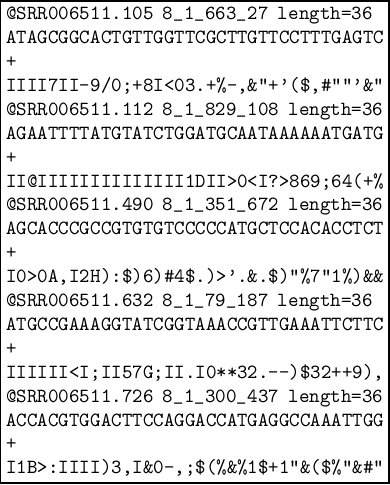
\includegraphics[width=0.5\textwidth]{ReadFile.jpg}
\end{center}
\caption{Example of a Sanger FASTQ file for input read data.}
\label{fig:fastq}
\end{figure}

\subsection{Splice Scores}
\label{sec:splicescoresfile}

As mentioned before, the splice site scores can be generated using an
appropriate tool such that
mGene~\cite{Schweikertetal09,Schweikertetal09b} or
ASP~\cite{Sonnenburgetal07}. If you would like to use your own splice
site predictions you can create files according to the Binary Signal 
Prediction Format (BSPF) described below: 

For each canonical acceptor ($AG$) and donor site ($GT$/$GC$)
\PALMapper{} expects a score. The data is organized in files for each
signal (acc/don) for each strand (+/-). The information on positions of
canonical splice sites and the corresponding scores lies in separate
files. Every chromosome or contig leads then to $8$ files (acc/don, +/-
and pos/score). The position and score files are raw binary files
containing the ordered positions and the scores. The positions are
stored as unsigned values and the scores as floats. Note that you have
to be careful when working in an inhomogeneous cluster environment
(endianness, data type size). The positions are 1-based and the
assignment of positions and their scores is as follows: The acceptor
score positions are the positions right after the $AG$ and the donor
score positions are the positions right on the $G$ of the $GT$ or
$GC$. For example:
\begin{center}
\begin{tabular}{ccccccccccc}
... & 3 & 4 & 5 & 6 & 7 & 8 & 9 & 10 & 11 & ... \\ 
... & w & g & t & x & y & z & a & g  & v  & ... \\
... &   & 0.2&  &   &   &   &   &    & 0.3 & ... 
\end{tabular}
\end{center}


\subsection{Alignment file}
\label{sec:samfile}
By default, the alignment file is encoded in a SAM format but the user
can alternatively choose between BED, an extended BED format (BEDx),
SHORE, and SAM formats using the option \texttt{-f}.

The SAM format used by \PALMapper{} is described below. For
complementary information, you should refer to
\url{http://samtools.sourceforge.net/}. Each row in SAM file describes
an alignment with the following fields:
\begin{enumerate}
\item \textbf{qname} - Query name (read id)
\item \textbf{flag} - Bitwise flag
\item \textbf{rname} - Reference sequence name (chromosome id) 
\item \textbf{pos} - 1-based leftmost position/coordinate of the
  clipped sequence 
\item \textbf{mapq} - Mapping Quality (phred-scaled posterior probability that the mapping
position of this read is incorrect). Field MAPQ considers pairing in
calculation if the read is paired. Providing MAPQ is recommended. If
such a calculation is difficult, 255 should be applied, indicating the
mapping quality is not available.
\item \textbf{cigar} -extended CIGAR string 
\item \textbf{mrnm} - Mate reference sequence name; “=” if the same as
  RNAME (set to * if no paired information)
\item \textbf{mpos} - 1-based leftmost Mate position of the clipped
  sequence (set to 0 if no paired information)
\item \textbf{isize} - inferred Insert SIZE (set to 0 if no paired information)
\item \textbf{seq} - query sequence
\item \textbf{qual} - query quality; ASCII-33 gives the Phred base quality
\item \textbf{tag} - Tag
\item \textbf{vtype} - Value type
\item \textbf{value} - match vtype (space allowed) 
\end{enumerate}

The fields \texttt{tag}, \texttt{vtype} and \texttt{value} are
concatenated and separated by a ":''. The possible tags
encountered in the output of \PALMapper{} are the following:\\

\begin{tabular}{|c|c|p{12cm}|}
\hline
{\bf Tag}&{\bf Type}&{\bf Description}\\
\hline
NM&i&Number of nucleotide differences (i.e. edit distance to the reference sequence)\\
\hline
H0&i&Number of perfect hits\\
\hline
XS&A&Strand information (for spliced alignments only)\\
\hline
Xe&i&Minimal exon length\\
\hline
XI&i&Maximal intron length\\
\hline
Xi&i&Minimal intron length\\
\hline
XC&Z&Non consensus splice site sequence in case of a spliced alignment
with a non-consensus splice site (with option \texttt{-non-consensus-search}) \\
\hline
XQ&i&Sum of mismatch qualities\\
\hline
XN&i&Number of exon(s)\\
\hline
ZS&f&\QP{} score for the alignment\\
\hline
AS&i&Alignment score generated by aligner (for \PALMapper{}, it
corresponds to \QP{} score multiplied by 100)\\
\hline
HI&i&Query hit index, indicating the alignment record is the i-th one stored in SAM\\
\hline
XD&f& \QP{} score difference between the alignment with the best
\QP{} score and the given one for the same query\\
\hline
Xd&i&Difference in terms of edit operations between the given
alignment and the alignment with the minimum number of edit operations
for the same query\\
\hline
\end{tabular}



\section{General settings}
\label{sec:settings}

\PALMapper{} offers a large set of parameters to run \GM{} and \QP{}
(see Tables~\ref{tab:palmapper_param} and~\ref{tab:qpalma_param}) and
running this tool with default parameters may lead to suboptimal
results. It is therefore important to monitor the alignment quality
using the provided evaluation and visualization tools before they are
used for further analysis. 

%%%%%%%%%%%%%%%%%%%%%%%%%%%%%%%
%% PALMapper options
%%%%%%%%%%%%%%%%%%%%%%%%%%%%%%%
\begin{table}[h!]
\begin{tabular}{p{3cm}p{6cm}cp{2cm}}
\hline
Option/Flag&Description&Default&Range\\
\hline
\texttt{-f}& output format&sam& [shore, bed, bedx, sam]\\
\texttt{-o}& output filename & stdout& STRING\\
\texttt{-u}& unmapped reads filename&/dev/null& STRING\\
\texttt{-z}& report a number of top scoring alignments&10&INT\\
\texttt{-a}& report all alignments as good as the best one&&\\
\texttt{-ar}& report a limited number of best alignments&0(all)&INT\\
\texttt{-r}& disable reverse alignment &&\\
\texttt{-h}& always perform alignment on entire read (implied for
spliced alignments)&&\\ 
\texttt{-d}& align gaps most right (most left) (ignored for spliced alignments)&&\\
\texttt{-w}& allow more gaps for best hit (ignored for spliced
alignments)&&\\ 
\texttt{-l}& seed length & index size & INT\\
\texttt{-threads}&maximal number of threads &4&INT\\ 
\texttt{-seed-hit -cancel-threshold}& number of hits of a seed that
lead to its ignoration &&INT\\
\texttt{-index-precache}& linearly read index file to fill caches&&\\
\texttt{-rtrim}&shortens the read until a hit is found or the minimal length is reached&&INT\\
\texttt{-polytrim}& trims polyA or polyT ends until a hit is found or
the minimal length is reached&&INT\\
\texttt{-rlim}& limit the number of reads for alignment&&INT\\
\texttt{-M}& max number of mismatches&3&INT\\
\texttt{-G}& max number of gaps&1&INT\\
\texttt{-E}& max edit operations&3&INT\\
\texttt{-m}& mismatch penalty&4&DOUBLE\\
\texttt{-g}& gap penalty &5&DOUBLE\\
\texttt{-v}& verbose &silent&\\
\hline
\end{tabular}
\caption{Description of the options that influence the general
  behaviour of \PALMapper{} (mostly for unspliced alignments).}
\label{tab:palmapper_param}
\end{table}


%%%%%%%%%%%%%%%%%%%%%%%%%%%%%%%
%% QPALMA options for alignment
%%%%%%%%%%%%%%%%%%%%%%%%%%%%%%%
\begin{table}[h!]
\begin{tabular}{p{3cm}p{6cm}clc}
  \hline
  Option/Flag&Description&Default&Range&Optional?\\
  \hline
\texttt{-S}& report spliced alignments (detailed options below)&&No\\
  \texttt{-qpalma}&file name with qpalma parameters&&STRING&No\\
  \texttt{-acc}&path name to acceptor splice site predictions&&STRING&No\\
  \texttt{-don}&path name to donor splice site predictions&&STRING&No\\
  \texttt{-no-ss-pred}&indicates that no splice site predictions should
  be used&&&Yes\\ 
  \texttt{-filter-splice -sites-top -perc}&trigger spliced alignments, if
  best read alignment covers putative splice site with score in the given top percentile &&[0-1],Float&Yes\\
  \texttt{-filter-max -mismatches}&trigger spliced alignment, if
  unspliced alignment has at least this many mismatches &0&INT&Yes\\
  \texttt{-filter-max-gaps}&trigger spliced alignment, if unspliced
  alignment has at least this many gaps&0&INT&Yes\\
  \texttt{-C}& min combined length&Auto&INT&Yes\\
  \texttt{-L}& min length of long hit&Auto&INT&Yes\\
  \texttt{-K}& min length of short hit&Auto&INT&Yes\\
  \texttt{-I}& longest intron length&Auto&INT&Yes\\ 
  \texttt{-EL}&Minimum segment length in spliced alignments&Auto&INT&Yes\\
  \texttt{-SA}& maximum number of spliced alignments per read &10&INT&Yes\\
  \texttt{-NI}& maximum number of introns in spliced alignments &Auto&INT&Yes\\
  \texttt{-CT}& distance to tolerate between hit and existing hit cluster&10&INT&Yes\\
  \texttt{-QMM}&number of matches required for identifying a splice site&5&INT&Yes\\
  \texttt{-qpalma-use-map -max-len}& limit the map extension up- and
  downstream to the given length &$10000$&INT&Yes\\ 
  \texttt{-report}& file for map reporting&&STRING&Yes\\
\texttt{-report-coverage -wig}&Output read coverage track in wriggle
format&&STRING&Yes\\
\texttt{-report-splice -sites}&Report splice sites with confidence not less than a threshold&&  FLOAT& Yes\\
\texttt{-report-splice -sites-top-perc}&Report splice sites with
confidence in top percentile&&[0-1], FLOAT& Yes\\
 \texttt{-report-gff-init}& initialize map with exons from GFF file&&STRING&Yes\\
  \hline
\end{tabular}
\caption{Description of the parameters influencing the spliced
  alignments in \PALMapper{} (only needed when option \texttt{-S} is given).}
\label{tab:qpalma_param}
\end{table}


\subsection{Influencing the General Behaviour}
The most important parameters that influence the sensitivity and
specificity of \PALMapper{} are \texttt{-M}, \texttt{-G} and
\texttt{-E} for specifying the maximal number of mismatches, gaps and
edit operations (mismatch or gaps) allowed in a reported alignment. We
often allow 4-6 mismatches for sequences of length 76 nt with at most
2 gaps.  However, reasonable results can already be obtained with just
1-2 mismatches and no gap (depending on the sequence quality and the
technology). Moreover, the options \texttt{-z}, \texttt{-a} and
\texttt{-ar} determine which alignments should be written into the
result files. In most cases, the setting \texttt{-z 1} will be
sufficient, where only the best alignment is determined and written to
the output file.  

\subsection{Spliced Alignments} 
There exist a few parameters that influence spliced alignments. First
of all, there are parameters, which influence when a spliced alignment
is triggered. This decision is made based on the number of mismatches
and gaps, the presence of strong splice site predictions for the best
unspliced alignment (options \texttt{-filter-max- mismatches},
\texttt{-filter-max-gaps}, and
\texttt{-filter-splice-site-top-perc}). Once the spliced alignment
routine is  triggered, the seed hits are analyzed and a full alignment
is performed for regions that are longer than a given length (option 
\texttt{-L}). This parameter should be set smaller than half of the
read length. The options \texttt{-I} and \texttt{-NI} determine the
maximal intron length and number that is allowed in spliced
alignments.  

\subsection{Using Report Maps to Improve Alignments}
\PALMapper{} implements a mechanism to exploit information from
existing annotations or from previous alignments to increase the
sensitivity of alignments. For instance, the option \texttt{-report-gff-init}
allows the user to specify a GFF file with known exons to guide and
improve spliced alignments. Similarly, the option
\texttt{-report-map-read} enables storing information of previously
mapped reads to improve the recognition of exonic regions in following 
spliced alignments. This option is often used in conjunction with
option \texttt{-report}, which specifies a file name to which the
mapping information is saved, and a two-step alignment approach: 1)
the reads are preliminarily aligned (for instance, unspliced or with
other stringent settings to increase the speed), and 2) a map file is
generated. This map file is used in the second step for a refined
spliced alignment. Finally, the options \texttt{-report-splice-sites} (and
\texttt{-report-splice-sites-top-perc}) can be used to exploit
computational splice site predictions to identify genomic regions to
which the reads should be aligned.  

\subsection{Settings for Faster Alignments} 
The following strategies will help to limit the computing time needed
for the alignment: 
\begin{itemize}
\item For very repetitive or large genomes the option
  \texttt{-seed-hit-cancel-threshold 1000} can help to reduce the
  alignment time, by ignoring seed hits which occur too often (more
  than 1,000 times) in the genome.
\item To reduce the number of spliced alignments performed
for one read, one may use the option \texttt{-SA} (e.g., \texttt{-SA 2}).
\item The seed length (option \texttt{-s} specified during index
  creation with pmindex) also determines the speed of the alignment:
  larger seeds have fewer hits in the genome and, hence, lead to
  faster alignment, but also to less sensitive results.
\item Reducing the maximal intron length (\texttt{-I}) will
also lead to quicker alignments.
\item To limit the size of the regions that are used for alignment
  that are inferred from the report maps (see above), there is a
  parameter: \texttt{-qpalma-use-map-max-len}. This parameter
  crucially influences the alignment speed, when the large parts of
  the genome are covered with reads or are annotated as exonic (set
  it, for instance, to 5000 to limit the alignment sequence length to
  2X5000 nt).  
\end{itemize}

It is useful to use the parameter \texttt{-rlim} to perform the  
alignment first on a small subset of the reads, for instance, 10,000, 
to estimate the time needed for aligning the reads.

\section{Internet Resources}
\url{http://www.fml.mpg.de/raetsch/suppl/palmapper}\\
\emph{\PALMapper{} project web-page.}\\
\url{http://www.fml.mpg.de/raetsch/suppl/palmapper/tutorial}\\
\emph{\PALMapper{} tutorial web-page.}\\
\url{http://www.fml.mpg.de/raetsch/suppl/qpalma}\\
\emph{\QP{} project web-page.}\\
\url{http://www.fml.mpg.de/raetsch/suppl/mgene}\\
\emph{\mGene{} project web-page.}\\
\url{http://www.fml.mpg.de/raetsch/suppl/splice}\\
\emph{\ASP{} project web-page.}\\
\url{http://ftp.tuebingen.mpg.de/pub/fml/raetsch-lab/software/}\\
\emph{http server for downloading \QP{}.}\\
\url{http://galaxy.fml.mpg.de/}\\
\emph{\Galaxy{} server.}\\

%
% Bibliography
% 

\begin{thebibliography}{1}

\bibitem[1]{DeBona08} 
  \newblock F.~De~Bona, S.~Ossowski, K.~Schneeberger, and G.~R{\"a}tsch.
  \newblock Optimal Spliced Alignment of Short Sequence Reads.
  \newblock {\em Bioinformatics}, 24(16):i174-i180, 2008.

\bibitem[2]{Palmapper} 
  \newblock G.~Jean, A.~Kahles, V.T.~Sreedharan, F.~De~Bona, and G.~R\"atsch.
  \newblock RNA-Seq Read Alignments with PALMapper.
  \newblock {\em Curr. Protoc. Bioinformatics}, 32:11.6.1-11.6.38, 2010.

\bibitem[3]{GenomeMapper}
  \newblock K.~Schneeberger, J.~Hagmann, S.~Ossowski, N.~Warthmann,
  S.~Gesing, O.~Kohlbacher, and D.~Weigel. 
  \newblock Simultaneous alignment of short reads against multiple genomes.
  \newblock {\em Genome Biology}, 10(9):R98, 2009.

\bibitem[4]{Tsochantaridis04} 
  \newblock I.~Tsochantaridis, T.~Hofmann, T.~Joachims and Y.~Altun.
  \newblock Support Vector Machine Learning for Interdependent and Structured Output Spaces.
  \newblock {\em Proceedings of the 16th International Conference on Machine Learning}, 2004.

\bibitem[5]{Schweikertetal09}
  \newblock G.~Schweikert, G.~Zeller, A.~Zien, J.~Behr, C.-S.~Ong, P.~Philips,
  A.~Bohlen, S.~Sonnenburg, and G.~R\"atsch.
  \newblock {mGene}: {A} Novel Discriminative Gene Finding System.
  \newblock {\em Genome Research}, 19:2133-2143, 2009.

\bibitem[6]{Schweikertetal09b}
  \newblock G.~Schweikert, J.~Behr, A.~Zien, G.~Zeller, S.~Sonnenburg, and G.~R\"atsch.
  \newblock mGene.web: a web service for accurate computational gene
  finding. 
  \newblock {\em Nucleic Acids Research}, 37(Suppl. 2):W312–W316, 2009. 

\bibitem[7]{Sonnenburgetal07}
  \newblock S.~Sonnenburg, G.~Schweikert, P.~Philips, J.~Behr, and
  G.~R{\"a}tsch. 
  \newblock Accurate splice site prediction using support vector machines.
  \newblock {\em BMC Bioinformatics}, 8(Suppl 10):S7, 2007.

\bibitem[8]{Galaxy1}
  \newblock D.~Blankenberg, J.~Taylor, I.~Schenck, J.~ He, Y.~Zhang,
  M.~Ghent, N.~Veeraraghavan, I.~Albert, W.~Miller, K.~Makova, R.~Hardison, and A.~Nekrutenko.
  \newblock A framework for collaborative analysis of ENCODE data: making large­scale analyses biologist-friendly.
  \newblock {\em  Genome Research}, 17(6):960–964, 2007. 

\bibitem[9]{Galaxy2}
  \newblock J.~Taylor, I.~Schenck, D.~Blankenberg, and A.~Nekrutenko.
  \newblock Using galaxy to perform large-scale interactive data
  analyses. 
  \newblock {\em Curr. Protoc. Bioinformatics}, 19:10.5.1-10.5.25, 2007. 

\bibitem[10]{Galaxy3}
  \newblock D.~Blankenberg, G.~Von~Kuster, N.~Coraor, G.~Ananda,
  R.~Lazarus, M.~Mangan, A.~Nekrutenko, J.~Taylor.
  \newblock Galaxy: A Web­Based Genome Analysis Tool for Experimentalists.
  \newblock {\em Curr. Protoc. Molecular Biology}, 89:19.10.1-19.10.21, 2010.


  



\end{thebibliography}
%
%
%
\end{document}
